\documentclass[a4paper,11pt, oldfontcommands]{memoir}
%\documentclass[b5paper,10pt,twoside]{memoir}
% Ved a4 format skal nedenst�ende nok justeres en del
\setlrmarginsandblock{3.5cm}{2.5cm}{*}
\setulmarginsandblock{3cm}{*}{1.2}

\usepackage[retainorgcmds]{IEEEtrantools}
\usepackage{graphicx}
\usepackage{pstricks,pst-node,pst-text,pst-3d}
\usepackage{marginnote}
\usepackage{array,booktabs,longtable}
\usepackage{url}
\usepackage{color}
\usepackage{array}
\usepackage{enumitem}
%\definecolor{webblue}{rgb}{0.0,0.05,0.45}
\definecolor{MyDarkBlue}{rgb}{0,0.08,0.45}
%\definecolor{webred}{rgb}{0.75,0,0}

\usepackage[T1]{fontenc}
\checkandfixthelayout
% ops�tning af pagestyles
\makepagestyle{book} % laver en ny tom pagestyle
\makeevenhead{book}{}{\small\sffamily\leftmark}{}
\makeoddhead{book}{}{\small\sffamily\rightmark}{}
\makeevenfoot{book}{\small\sffamily\thepage}{}{}
\makeoddfoot{book}{}{}{\small\sffamily\thepage}
\makeatletter

\makepsmarks{book}{%
\renewcommand\chaptermark[1]{%
\markboth{%
\ifnum \value{secnumdepth} > 1
\if@mainmatter % indenfor frontmatter er der intet kapitel nummer
\@chapapp\ \thechapter. \ % \@chapapp er lidt dum, se nedenfor
\fi
\fi
##1}{}}%
\renewcommand\tocmark{\markboth{\contentsname}{\contentsname}}%
\renewcommand\lofmark{\markboth{\listfigurename}{\listfigurename}}%
\renewcommand\lotmark{\markboth{\listtablename}{\listtablename}}%
\renewcommand\bibmark{\markboth{\bibname}{\bibname}}%
\renewcommand\indexmark{\markboth{\indexname}{\indexname}}%
\renewcommand\sectionmark[1]{\markright{##1}}%
\renewcommand\subsectionmark[1]{\markright{##1}}%
\renewcommand\subsubsectionmark[1]{\markright{##1}}%
}
\makeatother

\pagestyle{book}
% laver om p� plain stilen
\copypagestyle{plain}{book}
\makeevenhead{plain}{}{}{}
\makeoddhead{plain}{}{}{}

%**************** Headlines ****************************************************
% konfiguration af kapitel titel font samt fonte til sections
\renewcommand\chapnamefont{\Huge\bfseries\sffamily}
\renewcommand\chapnumfont{\chapnamefont}
%\renewcommand\chaptitlefont{\color{webred}\Huge\usefont{OT1}{phv}{bc}{n}\selectfont\raggedright}
\renewcommand\chaptitlefont{\Huge\usefont{OT1}{phv}{bc}{n}\selectfont\raggedright}
%\setsubsecheadstyle{\color{MyDarkBlue}\large\bfseries\sffamily\raggedright}
\setsubsecheadstyle{\large\bfseries\sffamily\raggedright}
%\setsubsubsecheadstyle{\color{webred}\Huge\usefont{OT1}{phv}{bc}{n}\selectfont\raggedright}
\setsubsubsecheadstyle{\Huge\usefont{OT1}{phv}{bc}{n}\selectfont\raggedright}
% Rule under headline.. (Underline section headlines med de 4 linier herunder) 
%\newcommand{\ruledsec}[1]{%
%\Large\usefont{OT1}{phv}{b}{n}\selectfont\raggedright #1 %\color{webred}\rule[15pt]{\textwidth}{1.0pt}} 
%\setsecheadstyle{\ruledsec} %ud-kommenter linie herunder
\setsecheadstyle{\Large\usefont{OT1}{phv}{b}{n}\selectfont\raggedright}

\usepackage{titlesec}
\usepackage{titletoc}
% Afstande mellem overskrifter og tekst
\titleformat{\subsection}
%{\color{MyDarkBlue}\usefont{OT1}{phv}{b}{n}\selectfont}{\thesubsection}{1em}{}
{\usefont{OT1}{phv}{b}{n}\selectfont}{\thesubsection}{1em}{}
\titleformat{\subsubsection}
%{\color{MyDarkBlue}\usefont{OT1}{phv}{b}{n}\selectfont}{\thesubsubsection}{1em}{}
{\color{black}\usefont{OT1}{phv}{b}{n}\selectfont}{\thesubsubsection}{1em}{}
\titlespacing{\subsection}{0pt}{15pt}{10pt}
\titlespacing{\subsubsection}{15pt}{15pt}{10pt}
\titlespacing{\section}{15pt}{35pt}{10pt}
%***********  section number in margin ****************************************
\makeatletter
\def\@seccntformat#1{\@ifundefined{#1@cntformat}%
{\csname the#1\endcsname\quad}% default
{\csname #1@cntformat\endcsname}% individual control
}
%\def\section@cntformat{\color{webred}\protect\makebox[0pt][r]{\thesection.\quad}}
\makeatother


% s�g for at hvis en \section el.lign. flyttes til en ny side
% da skal siden f�r ikke str�kkes
\raggedbottomsectiontrue
% justering af afsnitsnummerering og ToC dybde
\setsecnumdepth{subsubsection} % til og med
\maxsecnumdepth{subsubsection} % underligt koncept
%\settocdepth{subsection} %til og med
% nogle pakker man ofte anvender
\usepackage[ansinew]{inputenc} % eller ansinew hvis Windows
%*******************************************************************************
\usepackage[T1]{fontenc}
\usepackage{amsmath,amssymb}
\usepackage{mathtools}
\usepackage{graphicx}
\usepackage{fix-cm,fixltx2e}
\usepackage{soul}

\DeclareRobustCommand{\SetFourierSpace}{%
\fontdimen2\font=1.13\fontdimen2\font}
\sodef\an{}{0.13em}{0em}{0em} \sodef\ann{}{0.13em}{0.5em}{0em}
%******************************************************************************
\let\footruleskip\relax % for compatibility of memoir and fancyhdr
%% Use fancy chapter headers, with Jos Dingjan's modifications,
%% plus my own tweaks. This style is not part of teTeX,
%% so we are using a local (and renamed) copy. Reverted to original!
% \usepackage[Lenny]{fncychapleo}
\usepackage[Lenny]{fncychap}
\usepackage{fancyhdr}

% Setup af fncychap Lanny chapter header
\ChNameVar{\LARGE\usefont{OT1}{phv}{m}{n}\selectfont\raggedright}
\ChNumVar{\fontsize{75}{10}\usefont{OT1}{cmr}{m}{n}\selectfont\raggedright}
\ChTitleVar{\Huge\usefont{OT1}{phv}{bc}{n}\selectfont\raggedright}

%*******************************************************************************

\makeatletter
\newcommand\figcaption{\def\@captype{figure}\caption}
\newcommand\tabcaption{\def\@captype{table}\caption}
\makeatother

%\newenvironment{narrow}[2]{%
%\begin{list}{}{%
%\setlength{\topsep}{0pt}%
%\setlength{\leftmargin}{#1}%
%\setlength{\rightmargin}{#2}%
%\setlength{\listparindent}{\parindent}%
%\setlength{\itemindent}{\parindent}%
%\setlength{\parsep}{\parskip}}%
%\item[]}{\end{list}}

\newlength{\marginwidth}
\setlength{\marginwidth}{2.0\oddsidemargin} %bredden af billeder ud i margin'en

% Picture Handling
\usepackage{subfig}
\usepackage[leftcaption]{sidecap}
%\usepackage{varioref} %For smarte referencer med \vref istedet for \ref
\usepackage[hidelinks]{hyperref}
\usepackage{cleveref}
\usepackage{calc}% auto udregn

\usepackage{tikz}
\usepackage{pgf-umlsd}
\usetikzlibrary{arrows, chains}

\graphicspath{{figures/}}
\sidecaptionvpos{figure}{t} %sidecaption aligned med toppen af billede
\usepackage{caption}
%\DeclareCaptionFont{red}{\color{webred}}
\DeclareCaptionFont{defaultCapFont}{\color{black}}
\captionsetup{singlelinecheck=false,font=footnotesize,labelfont={bf,defaultCapFont},format=hang}

\DeclareCaptionFormat{llap}{\llap{#1#2}#3\par}
\strictpagechecktrue
\makeatletter
\DeclareRobustCommand*{\bfseries}{%
  \not@math@alphabet\bfseries\mathbf
  \fontseries\bfdefault\selectfont
  \boldmath
}
\makeatother

% andre pakker og konfigurationer
\usepackage{makeidx}
\usepackage{mflogo} 
\makeindex % hvis man anvender s�dan en

%\renewcommand*{\cftchaptername}{Chapter\space}
\renewcommand*{\cftchaptername}{}
\renewcommand*{\cftfigurename}{Fig.\space}
\renewcommand{\contentsname}{Table of Contents}
\renewcommand*\abstractname{Summary}

%\includeonly{Loadbalancing} %Hvis man ikke vil kompilere det hele hver gang
\begin{document}
\frontmatter

\selectlanguage{english} 
\begin{abstract}
Wind energy is widely recognized as one of the most cost efficient renewable energy sources. 
%Because of this wind farms are increasing in size and power production. 
%Because of this wind farm size and power production is increasing.
Because of this wind farm size and power production steadily increases.
%, in order to accommodate the rising need for energy from renewable sources. 
%The number of turbines in a single wind farm can reach more than 500.
Control of the increasing number of turbines in wind farms is becoming problematic.
%
The traditional hierarchical control approach with central control points responsible for regulation of turbine power production does not scale well with the number of turbines, and contains single points of failure.
%
The present thesis aims to decentralize the control of turbines in order to increase the number of turbines handled per control unit and remove single points of failure. 
%
%This is done by letting each turbine regulate it's own power production in accordance with the power production of all other turbines in the wind farm.
This is achieved by letting the turbines regulate power production themselves, while cooperating to reach the power production setpoint of the wind farm. Data storage and aggregation, load balancing and communication are identified as key areas for decentralization.
%In place of the hierarchical control approach the aim is to decentralize the control of turbines in a wind farm by letting each turbine control it's own power production in accordance with the power production of all other turbines in the wind farm.
%In place of the hierarchical control approach this thesis aim to let every turbine control itself in accordance with the power production of other turbines, in effect decentralizing the control of the wind farm.
MongoDB, Linux Virtual Server and RTI Connext Data Distribution Service for Real-Time Systems (DDS) has been identified as optimal components for handling these key areas. 
A decentralized prototype of a wind farm, performing power regulation using RTI Connext DDS for communication is presented.
The prototype is evaluated and compared to a prototype of an existing Siemens Wind Power wind farm. Within the limits set by the test environment, the decentralized prototype outperforms the prototype of an existing Siemens Wind Power wind farm, as the decentralized prototype is shown to scale constant with the number of turbines.
\end{abstract}

\selectlanguage{danish} 
\begin{abstract}
Vindenergi er bredt anerkendt som en af de mest omkostningseffektive vedvarende energikilder.
Derfor stiger vindmølleparkers størrelse og elproduktion støt.
Kontrol af det stigende antal møller i en vindmøllepark er problematisk.
Den traditionelle hierarkiske kontrol tilgang med centrale kontrolpunkter, der har ansvar for at regulere turbinernes elproduktion skalerer ikke godt med antallet af turbiner, og introducerer single points of failure.
Det nærværende speciale har til formål at decentralisere kontrollen af turbiner for at øge antallet af turbiner håndteret per kontrol enhed og fjerne single points of failure.
Dette opnås ved at lade turbinerne regulere deres elproduktion selv, mens de samarbejder for at nå vindmølleparkens sætpunkt for elproduktion.
Data lagring og indsamling, load balancer og kommunikation bliver identificeret som nøgleområder med hensyn til decentralisering.  
MongoDB, Linux Virtual Server og RTI Connext Data Distribution Service for Real-Time Systems (DDS) er blevet identificeret som værende optimale komponenter til håndtering af disse nøgleområder.
En decentraliseret prototype af en vindmøllepark, der udfører strøm regulering ved brug af RTI Connext DDS til kommunikation, bliver præsenteret. 
Prototypen bliver evalueret og sammenlignet med en prototype af en eksisterende Siemens Wind Power vindmøllepark. 
Inden for grænserne sat af det benyttede testmiljø, udkonkurrerer den decentraliserede prototype protypen af en eksisterende Siemens Wind Power vindmøllepark, da det bliver påvist at den decentraliserede prototype skalerer konstant med antallet af turbiner.

\end{abstract}
\selectlanguage{english} 

\cleartorecto
\tableofcontents

\mainmatter
\chapter{Introduction}

A Distributed Computing System is a concept where a network of multiple nodes works on a single problem. In Distributed Computing a problem is divided into smaller parts and solved by different notes. The nodes can be physically close, connected via a local network, or geographically distant, connected by a wide area network. The goal of a distributed computing is to make such a node network act as a single computer.

\begin{figure}
	\centering
	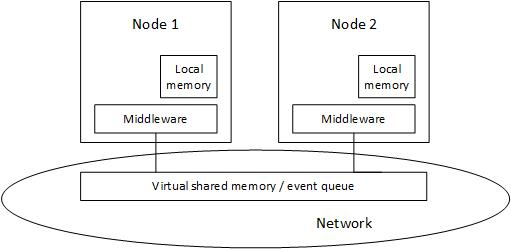
\includegraphics[width=0.8\textwidth,natwidth=610,natheight=642]{DistributedComputingSystemWith2nodes.jpg} 
	\captionsetup{format=plain,font=footnotesize,labelfont={bf,red},labelsep=quad,singlelinecheck=no}
	\caption[Distributed Computing System with 2 nodes]{
		\label{fig:distributedCoputingSystem} 
		\footnotesize{%
			A Distributed Computing System with 2 nodes.
		}
	}
\end{figure}

Figure \cref{fig:distributedCoputingSystem} illustrates the idea of a distributed computing system. Nodes 1 and 2 shares some virtual memory and/or event queue. The Middleware is a handles communication between the nodes and ensures the virtual memory is consistent throughout the network. The shared virtual memory is transparent to each node. 

Distributed systems offer many benefits over centralized systems including the following:
\begin{itemize}
	\item Scalability: It is easy to add notes to the system, should the size of the system increase.
	\item Redundancy: Several nodes can provide the same service, so if a node crashes, there are many to replace it. Additionally, from a cost perspective, each node does not have to be expensive, because many smaller nodes can be used as replacement.
\end{itemize}

\section{Thesis motivation}

\subsection{Siemens case}
Siemens Wind Power is among the leading windmill manufacturers in the world. 
Siemens builds wind farms of different sizes ranging form single mills to well above one hundred windmills \cite{simensOffShoreProjects, simensOnShoreProjects}.

In the current setup (see \cref{fig:currentSiemensSetup}) the Park Monitor is a central component and a SPOF (single point of failure).
The system is running on windows with a MSSQL database in the Park Monitor and MySQL on the windmills them self.
The windmills, Park Monitor and Park Regulator is connected with a gigabit network, witch currently has plenty of extra capacity.
The system handles more than 50 control points and 200 measurement points, and samples these every 50 ms.
The Park regulator is associated with the transformer station and regulated the power production when needed.
This component currently has a less than optimal work flow see \cref{fig:dataComputationSequence}.

Siemens has a need for their system to scale better and provide increased redundancy to avoid these SPOF's.
Siemens has a vision of removing the Park Monitor component and make it into a distributed system, distributed among the windmills (see \cref{fig:futureSiemensSetup}).
Also Siemens would like to look for ways to optimise the calculations done by the Park Regulator, 

\begin{figure}
	\centering
	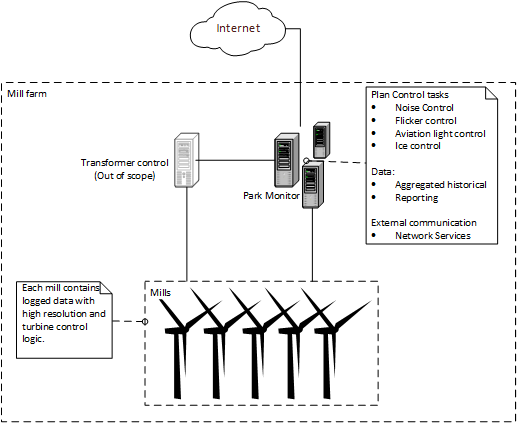
\includegraphics[width=0.7\textwidth,natwidth=610,natheight=642]{SystemOverviews.png} 
	\captionsetup{format=plain,font=footnotesize,labelfont={bf,red},labelsep=quad,singlelinecheck=no}
	\caption[Illustrates the current Siemens windmill farm setup]{
		\label{fig:currentSiemensSetup} 
		\footnotesize{%
			This figure illustrates the current Siemens windmill farm setup.
		}
	}
\end{figure}

\begin{figure}
	\centering
	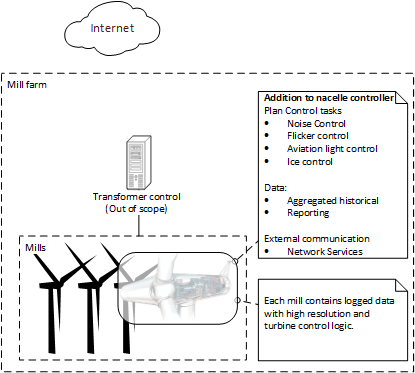
\includegraphics[width=0.7\textwidth,natwidth=610,natheight=642]{SystemOverviewsFuture.png} 
	\captionsetup{format=plain,font=footnotesize,labelfont={bf,red},labelsep=quad,singlelinecheck=no}
	\caption[Illustrates the future Siemens windmill farm setup]{
		\label{fig:futureSiemensSetup} 
		\footnotesize{%
			This figure illustrates the future Siemens windmill farm setup.
		}
	}
\end{figure}

\begin{figure}
	\centering
	\begin{sequencediagram} %Created using pgf-umlsd
		\newthread{reg}{:Park Regulartor}
		\newinst[2]{mill}{:Mill}
	
		\begin{sdblock}{each mill}{}
			\mess[1]{reg}{getCurrentStatus}{mill}
			\mess[1]{mill}{status}{reg}	
		\end{sdblock}
		
		\begin{call}{reg}{calculateAllSetpoints()}{reg}{}
		\end{call}
	
		\begin{sdblock}{each mill}{}
			\mess[1]{reg}{setNewSetpoint}{mill}
		\end{sdblock}
					
	\end{sequencediagram}

	\captionsetup{format=plain,font=footnotesize,labelfont={bf,red},labelsep=quad,singlelinecheck=no}
	\caption[Regulator calculation sequence]{
		\label{fig:dataComputationSequence} 
		\footnotesize{%
			Regulator calculation sequence.
		}
	}
\end{figure}
















\subsection{et eller andet}

Today windmills in windmill farm at Siemens are equipped with a computer for regulation, data and communication purposes. Every windmill are connected to a single server that aggregates data, perform calculations, store data and handle communication with the outside world. At Siemens up to 8 of theses servers are present pr. windmill farm and they pose the following problems:
\begin{itemize} 
	\item Single point of failure. Should a server fail, a part of the windmill farm will become unavailable.
	\item Low scalability. The servers does not scale with the number of windmills.
	\item Up performance of park regulator.
\end{itemize}

Therefor Siemens wishes to remove the servers by making every windmill farm a Distributed Computing System, utilizing free capacity of the computers already residing in every windmill. This would up the redundancy and scalability and the remove possibility of a single point of failure. A windmill farm must serve as single server which means ease of access must be maintained even though computation and data is distributed. This means routing traffic to a windmill with free capacity through a single interface, without external systems being aware of it.

% Today windmills in windmill farm are connected to a single server that aggregates data, perform calculations, store data and handle communication with the outside world. These servers do not scale well with the size of the windmill farm, and they are a single point of failure. Therefor Siemens wishes to remove the servers by utilizing free capacity of the computers already residing in every windmill. 
%Currently there is some limited redundancy in data and availability but this could be greatly improved by distributing data and communication to the windmills. 
%Ease of access must be maintained even though computation and data is distributed. 
%This means routing traffic to a windmill with free capacity through  a single interface.

\section{Thesis aim}

The purpose of this thesis is to design, implement and evaluate a framework and associated tools for distributed computing systems development. The case from Siemens Windpower is an example of a production environment where the framework could be utilized. The goal is not to make a framework that is specific to the Siemens case but to make a general framework for this and similar cases. 

This framework must be able to handle computation distributed on several nodes, communication between those nodes and distribution of data. 

The framework will be evaluated with regards to the existing Siemens solution using the following parameters: ... and will be done by comparing results obtained from a protocol 


%\begin{itemize}
%	\item How do we distribute a database and computation across a production environment in the best possible way?
%	\item How do we define and measure performance?
%	\item Can it provide data redundancy and outperform current systems?
%	\item How many windmills are needed before it makes sense to makes sense to distribute the server?
%\end{itemize}
%
%We aim to investigate the possibility of making a framework and associated tools for developing a distributed system. 
%This framework must be able to handle computation distributed on several nodes, communication between those nodes and distribution of data. 
%The communication can be built on top of existing standards as for instance DDS. Data distribution can be built using existing systems like MongoDB. 
%Distribution of computation tasks is the main research area and will be the focus of this thesis.
%
%In order to achieve distributed computation on several nodes the framework must be able to perform load balancing and control the distribution of tasks on the nodes in the system. 
%Furthermore the framework must have a single interface for control of, and interaction with, all the nodes.  
%The goal is to create a test system, that can distribute and perform tasks but also to be able to plan ahead of time and know if there is available computation time.
%
%The case from Siemens Windpower is an example of a production environment where the framework could be utilized. 
%Our goal is not to make a framework that is only  specific for this case but to make a general framework for this and similar cases.

\section{Approach}

\section{Outline}
The remainder of this thesis is organized into the following chapters...

\section{Audience}
This thesis is aimed at an audience with a basic knowledge of...

%\subsection{Siemens case}
Siemens Wind Power is among the leading windmill manufacturers in the world. 
Siemens builds wind farms of different sizes ranging form single mills to well above one hundred windmills \cite{simensOffShoreProjects, simensOnShoreProjects}.

In the current setup (see \cref{fig:currentSiemensSetup}) the Park Monitor is a central component and a SPOF (single point of failure).
The system is running on windows with a MSSQL database in the Park Monitor and MySQL on the windmills them self.
The windmills, Park Monitor and Park Regulator is connected with a gigabit network, witch currently has plenty of extra capacity.
The system handles more than 50 control points and 200 measurement points, and samples these every 50 ms.
The Park regulator is associated with the transformer station and regulated the power production when needed.
This component currently has a less than optimal work flow see \cref{fig:dataComputationSequence}.

Siemens has a need for their system to scale better and provide increased redundancy to avoid these SPOF's.
Siemens has a vision of removing the Park Monitor component and make it into a distributed system, distributed among the windmills (see \cref{fig:futureSiemensSetup}).
Also Siemens would like to look for ways to optimise the calculations done by the Park Regulator, 

\begin{figure}
	\centering
	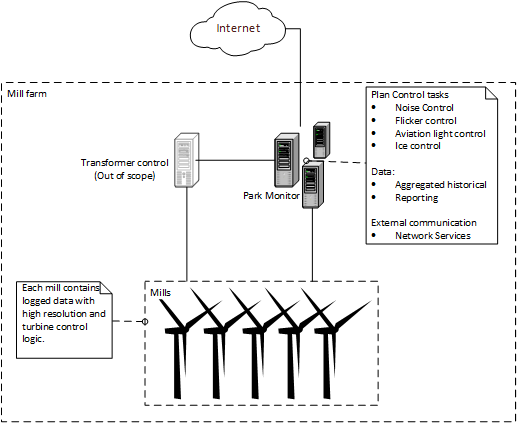
\includegraphics[width=0.7\textwidth,natwidth=610,natheight=642]{SystemOverviews.png} 
	\captionsetup{format=plain,font=footnotesize,labelfont={bf,red},labelsep=quad,singlelinecheck=no}
	\caption[Illustrates the current Siemens windmill farm setup]{
		\label{fig:currentSiemensSetup} 
		\footnotesize{%
			This figure illustrates the current Siemens windmill farm setup.
		}
	}
\end{figure}

\begin{figure}
	\centering
	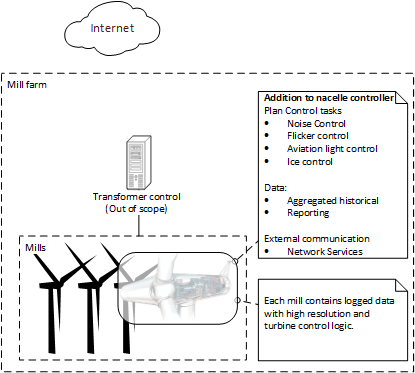
\includegraphics[width=0.7\textwidth,natwidth=610,natheight=642]{SystemOverviewsFuture.png} 
	\captionsetup{format=plain,font=footnotesize,labelfont={bf,red},labelsep=quad,singlelinecheck=no}
	\caption[Illustrates the future Siemens windmill farm setup]{
		\label{fig:futureSiemensSetup} 
		\footnotesize{%
			This figure illustrates the future Siemens windmill farm setup.
		}
	}
\end{figure}

\begin{figure}
	\centering
	\begin{sequencediagram} %Created using pgf-umlsd
		\newthread{reg}{:Park Regulartor}
		\newinst[2]{mill}{:Mill}
	
		\begin{sdblock}{each mill}{}
			\mess[1]{reg}{getCurrentStatus}{mill}
			\mess[1]{mill}{status}{reg}	
		\end{sdblock}
		
		\begin{call}{reg}{calculateAllSetpoints()}{reg}{}
		\end{call}
	
		\begin{sdblock}{each mill}{}
			\mess[1]{reg}{setNewSetpoint}{mill}
		\end{sdblock}
					
	\end{sequencediagram}

	\captionsetup{format=plain,font=footnotesize,labelfont={bf,red},labelsep=quad,singlelinecheck=no}
	\caption[Regulator calculation sequence]{
		\label{fig:dataComputationSequence} 
		\footnotesize{%
			Regulator calculation sequence.
		}
	}
\end{figure}















%\chapter{Dedication}




\chapter{State of the art}
As mentioned in \cref{chap:intro} there are a number of large scale wind park projects, but not many give a hint of their underlying software architecture.
One way to get an idea of how the systems are structured could be by looking at the control algorithms they use.

%\section{Control}
%One area that is still open for optimization is the control of turbines both as a single unit but also as a park. 
%Calculating the perfect position for each turbine such that the global power production setpoint is reached is a very hard problem.
%The algorithms must take a lot of parameters into account as for instance noise produced by the wings, certain speeds where the wear and tear of the turbine is high and the position of other turbines so the wake created by one turbine does not reduce the performance of other turbines unnecessarily.
%Furthermore every turbines maximum power production and current power production must also be taken into account.
%Several approaches has been tested as described in the following subsections. %TODO: Rewrite,

\section{Aeolus}
The Aeolus project was a large scale EU supported project which lasted from may 2008 to april 2011. It included project partners from 
Aalborg University, Industrial Systems and Control Ltd in Glasgow, University of Zagreb, Energy Research Centre of the Netherlands and Vestas Wind Systems A/S.
The main objectives of the project was to research and develop predictions of flows and incorporate data from a network of sensors, as well as research and develop control paradigms that acknowledges the uncertainty in the modelling and dynamically manages the flow resource in order to optimise specific control objectives.
The project is relevant to this thesis because several approaches to control of a wind park was evaluated.

\subsection{Hierarchical control}
The hierarchical approach uses local control on the turbine level and global control on the wind farm level\cite{HeirarchicalWindFarmControl}.

Setpoints for the global output of the wind farm are received by the controller on the wind farm level.
So is the output for each turbine and the maximum available output for each turbine.
The global controller calculates setpoints for each turbine based on the global setpoint and each turbines current and possible output.

The controllers on turbine level is responsible for reaching the setpoint calculated by the global controller as well as making each turbine reach the setpoint in the most optimal manner(gearing, avoid ice over, avoid oscillation).

The hierarchical approach is the current approach used in the Siemens case.

\subsection{Decentralized feed-forward control}
The decentralized feed-forward approach\cite{DecentralisedFeedforwardControlOfWindFarms} takes advantage of the fact that turbines are placed in a farm by letting upwind turbines feed wind data to downwind turbines. 
This allows downwind turbines to make adjustments to their production in order to exploit the coming wind in the best way.
Furthermore a restricted communication model is used allowing turbines only to communicate with their neighbors.

Using this decentralized feed-forward approach to control a wind farm can help even out the output of the farm since downwind turbines has additional information regarding wind speed to come to act upon. If upwind turbines power production is also a part of the feed-forward package downwind turbines may also be able to regulate overall wind farm production by evening out spikes from upwind turbines.
In addition by only communicating with neighboring turbines in order to achieve improvements in output the need for a centralized node is alleviated.

%\subsection{Game theory control}
%A new approach to control of wind farms is to utilize game theory\cite{AModelFreeApproachToWindFarmControl}.
%The turbines in a farm must cooperate to reach the desired goal of a chosen output current.
%The game theory approach use an iterative learning algorithm that converges against the optimal output after n iterations.
%According to the above referenced article improvements on up to 25\% is possible compared to other algorithms currently in use.
\chapter{Analysis}
% !TeX spellcheck = en_US
\chapter{Prototype development}
The prototype in this project will consist of X virtual machines.



\section{Platform}

Windows
Pro
\begin{itemize}
	\item Well known to most people (easy to get going) 
	\item 
\end{itemize}

Bad
\begin{itemize}
	\item expensive
\end{itemize}



Linux
Pro
\begin{itemize}
	\item Market leader [?] Need Source
	\item Linux Virtual server
	\item Linux Containers
	\item Open source / free
	\item More configurable with respect to scheduler (non preemptive (default), preemptive voluntary, RT ) 
	\begin{itemize}
		\item \url{http://www.linuxtopia.org/online_books/linux_kernel/kernel_configuration/re152.html}
		\item \url{http://stackoverflow.com/questions/5174955/what-is-voluntary-preemption}
		\item \url{http://lwn.net/Articles/146861/}
		\item \url{https://www.osadl.org/uploads/media/ECE-2011-09.pdf}
		\item \url{http://www.linux.com/news/featured-blogs/200-libby-clark/710319-intro-to-real-time-linux-for-embedded-developers}
								
	\end{itemize}
\end{itemize}



%user: shared
%password: windfarm

%https://forums.virtualbox.org/viewtopic.php?f=6&t=63556&start=165
 

The prototype is split int the following 3 parts:
\begin{itemize}
	\item DataSimulator
	\item HPPP component
	\item Monitor (UI component)
	\end{itemize}


\begin{tikzpicture} 
\begin{umlseqdiag} 
	\umldatabase{DB} 
	\umlmulti{DataSimulator}
	\umlmulti{Regulation Controller}
	\umlmulti{Monitor}
	\begin{umlcall}[op=getAlldata(), type=asynchron, return=0]{DB}{DataSimulator}
		\begin{umlfragment}[type=ForAll, label=Samples, inner xsep=8, fill=white!10]
			\begin{umlcall}[op=Simumlation data, type=synchron, return=setpoint]{DataSimulator}{Regulation Controller}
			
			\end{umlcall}
			\begin{umlfragment}[type=opt, fill=white!10]
				\begin{umlcall}[op=UpdateUI(), type=asynchron, return=0]{DataSimulator}{Monitor}
				\end{umlcall}
			\end{umlfragment}
		\end{umlfragment}


	\begin{umlcall}[op=saveData(), type=asynchron, return=0]{DataSimulator}{DB}
	\end{umlcall}	
	\end{umlcall}
	
	
\end{umlseqdiag} 
\end{tikzpicture}


% !TeX spellcheck = en_US
\chapter{Discussion}

\section{Number of turbines and the impact on regulation cycle time in the decentralized solution}
This section addresses the \ref{PS:Q:Performance} problem of \cref{sec:problemStatement}. In the current Siemens system the regulation cycle time of a single Park Pilot scales linearly with the number of turbines.
The aim of the decentralized solution is to detach the regulation cycle time from being dependent on the number of turbines. 
Looking at \cref{fig:exp:decen:turbines} in \cref{chap:results} we see that the decentralized solution is almost independent on the number of turbines.
From 5 to 65 turbines the regulation cycle time is nearly constant on $20 ms$ with very little variation in the dataset and moderate extreme values.
The constant regulation cycle time is caused by the fact that the regulation cycle in the decentralized system is not forced to wait for data before running the regulation algorithm because data is continually shared between turbines.

When looking at regulation cycle time of the decentralized solution the number cache reads.
As explained in \cref{sec:exp:performance} a cache read happens when a turbine does not provide a new turbine state package before the next regulation cycle is started.
This forces the regulation cycle to use old data read from cache.
Looking at \cref{fig:exp:decen:turbines_cache} we see that the average number of cache reads in the decentralized solution are below 5 and increasing slightly until we reach 65 turbines. From there the number of cache reads increases exponentially.

The increase in regulation cycle time and cache reads when the number of turbines reaches 65 can be explained by the fact that the network equipment of the test setup is approaching maximum throughput capacity which may cause lost or delayed network packages.
Since regulation cycle time in the decentralized system is dependent on the reception time of the oldest turbine state package as explained in \cref{sec:exp:performance} the loss or delay of network packages has a direct impact on regulation cycle time.
Similarly lost or delayed network packages increases the use of cached data. The increased regulation cycle time and cache reads are thus not a limitation of the decentralized solution but a limitation imposed by the test setup.

Disregarding the limitations imposed by the test setup we see that the regulation cycle time is nearly constant while the number of cache reads increases slowly with a factor of around 1 cache read for every 30 turbines added.

The number of cache reads can be reduced by increasing the regulation cycle time as presented in \cref{fig:exp:decen:sleep-cache}.
Thus the factor deciding the time of the regulation cycle is the maximum number of average cache reads accepted for a single regulation cycle.

\section{Comparison of decentralized solution and centralized solution}

\section{Comparison of decentralized and current Siemens system}

\begin{itemize}
	\item Test parameters: Our system vs Siemens system?
	\item Redundancy, up time, scalability...
	\item Solved problems (i.g. Single point of failure)
\end{itemize}
\chapter{Conclusion}

%\chapter{Literature Review}\label{chapter1}


%\chapter{Your Title}

\section{You Can Underline This Headline - See Preamble }

\subsection{A Smaller Headline}

%Below you will find three different examples on figure configurations  
%\begin{figure}[t]
%\centering
%\includegraphics[trim=10 0 10
%10,clip,keepaspectratio,width=\textwidth]{Preprocessing/xt_and_yt2} 
%\vspace*{5mm}
%\includegraphics[trim=10 0 10
%10,clip,keepaspectratio,width=\textwidth]{Preprocessing/spectral4} 
%\caption[Spectral analysis of a signature]{The figure illustrates the $y$-coordinate and the $x$-coordinate as a function of time. The figures are contracted on the time axis, which means that time segments with pen ups have been removed. Below, a spectral analysis of the signals is illustrated.}
%\label{fig:xt_and_yt}
%\end{figure}

%\begin{SCfigure}[][t] 
%\includegraphics[trim=10 0 20
%10,clip,keepaspectratio,width=0.6\textwidth]{Preprocessing/Signature2} 
%\captionsetup{format=plain,font=footnotesize,labelfont={bf,red},labelsep=quad,singlelinecheck=no}
%\caption[A signature example from the SVC2004 database]{\label{fig:signature} \footnotesize{This figure illustrates one of the signatures of the SVC2004 database. The beginning of every stroke is marked with a red circle, and the order of stroke execution is indicated by the matching numbers.}} 
%\end{SCfigure}


%\begin{figure}[tb]
%\begin{narrow}{-\marginwidth}{-\marginwidth}
%\includegraphics[keepaspectratio,width=\linewidth]{Preprocessing/Pos_Covar2}
%\vspace*{3mm}
%\includegraphics[keepaspectratio,width=\linewidth]{Preprocessing/Neg_Covar2}
%\captionsetup{singlelinecheck=false,font=footnotesize,labelfont={bf,red},format=plain}
%\caption[Correlation of 2D Gaussians]{The upper figures illustrates positive correlation between two normal distributions, while the lower figures illustrate negative correlation. The covariance is a measure of the linear relationship between the two components}
%\label{fig:EX_Covar}
%\end{narrow}
%\end{figure}





%\chapter{Conclusion}

\appendix
\addtocontents{toc}{\protect\setcounter{tocdepth}{0}}
\appendixpage
%\appendix
\addtocontents{toc}{\protect\setcounter{tocdepth}{0}}
\chapter{Deriving Max Likelihood for GMM/HMM Using the EM Algorithm}\label{appendix1}

%%\appendix
\chapter{Implementation of the Baum-Welch Algorithm}\label{appendix2}

%%\appendix
%\addtocontents{toc}{\protect\setcounter{tocdepth}{0}}
\chapter{Feature Extraction for the HMM}\label{appendix3}


\backmatter
\renewcommand{\bibsection}{%
\chapter{\bibname}
\prebibhook}
\bibliographystyle{plain} % eller en anden stil
%\bibliographystyle{IEEEbib}
\bibliography{my-bibliography-file}
%\bibliography{minbib}
% print indeks hvis det er noget man anvender

\clearpage
\listoffigures
\clearpage
\listoftables
\chapter{Nomenclature}


\begin{table}[ht]
\captionsetup{singlelinecheck=false,labelsep=newline,justification=centering,font=footnotesize,labelfont={bf,defaultCapFont},format=plain}
\caption[Nomenclature]{\textsc{\ann{The Terminology used in this Thesis}}} % title of Table
\centering % used for centering table
\begin{tabular}{l l l} % centered columns (4 columns)
\hline\hline\\ %inserts double horizontal lines
 Acronym & Description \\ [0.5ex] % inserts table
%heading
\hline\\ % inserts single horizontal line

	SPOF & Single point of failure \\
	WPS &  Wind Power Supervisor\\[1ex] % [1ex] adds vertical space

\hline %inserts single line
\end{tabular}
\normalsize
\label{table:nomenclature} % is used to refer this table in the text
\end{table}




\printindex
\end{document}



